This section presents the methodological procedures used to develop and evaluate the proposed approach.  
The method, illustrated in Figure~\ref{fig:method}, was structured in four main stages: (i) materials, (ii) preprocessing, (iii) feature extraction and model training, and (iv) performance evaluation.  
Each stage is described in detail in the subsections below.

\begin{figure}[H]
	\centering
	\makebox[\linewidth][l]{%
		\hspace*{-1cm}
		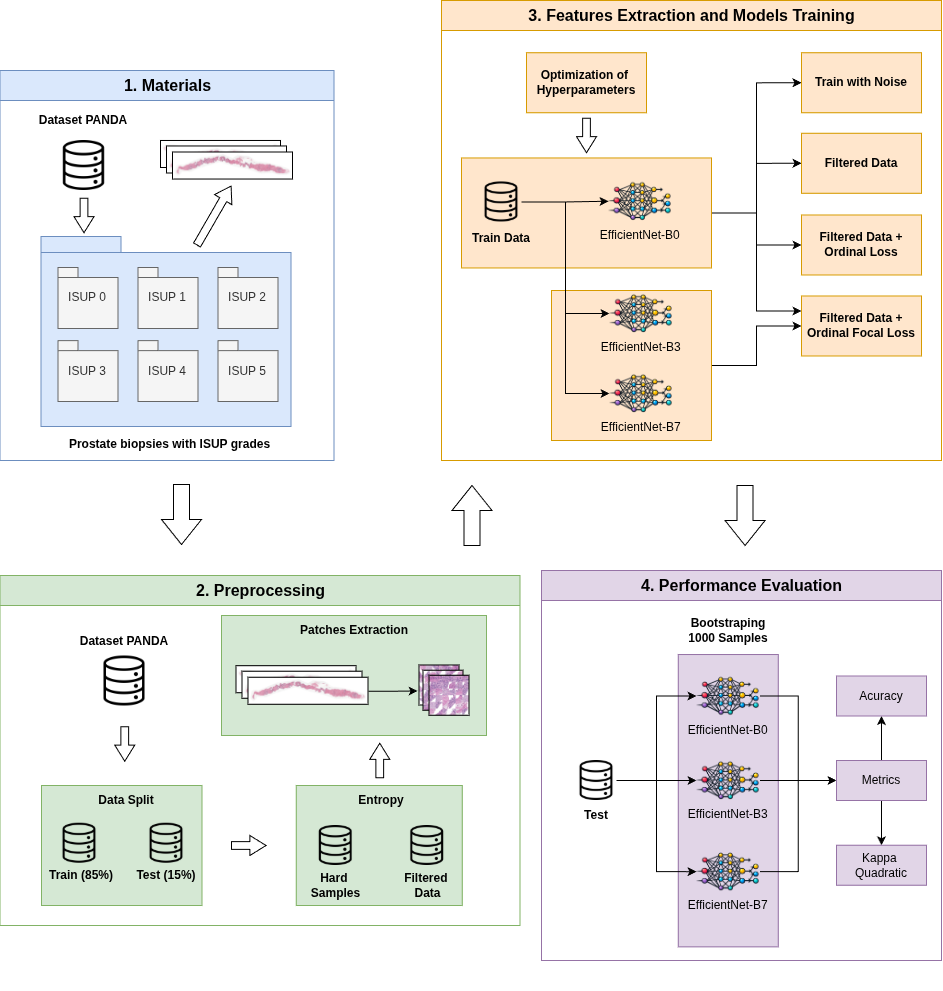
\includegraphics[width=1\linewidth]{images/method_bio.png}
	}
	
	\caption{Proposed Method}
	\label{fig:method}
\end{figure}

\subsection{Materials}
\label{sub:data}

In this study, the PANDA (\textit{Prostate Cancer Grade Assessment}) dataset was used, which consists of approximately 10,616 whole-slide histopathological images of prostate biopsies \cite{ref-panda2020}.  
This dataset was provided as part of the PANDA challenge on the Kaggle platform and has been widely used in research on automatic prostate cancer grading.  

The images in the dataset are annotated with Gleason scores and Gleason grades, providing clinical labels used for disease grading.  
In this study, only the public version of the dataset was used, without access to the private test set provided during the challenge.  

The data were collected from two medical centers, \textit{Radboud University Medical Center} and \textit{Karolinska Institute}, introducing institutional variability in the images.  
This variability is associated with differences in slide preparation protocols, scanning procedures, and annotation criteria, thereby making the experimental setting more closely resemble real clinical practice.  

Additionally, the dataset contains inherent noise from the slide acquisition and annotation processes.  
Visual artifacts include pen marks made by pathologists during slide analysis, as illustrated in Figure~\ref{fig:pen_mask}.  
There are also noise sources related to labeling, such as disagreement among annotators in assigning histopathological grades.  
These factors increase the complexity of the automatic classification task and reflect challenges present in digital pathology practice.

\begin{figure}[H]
	\centering
	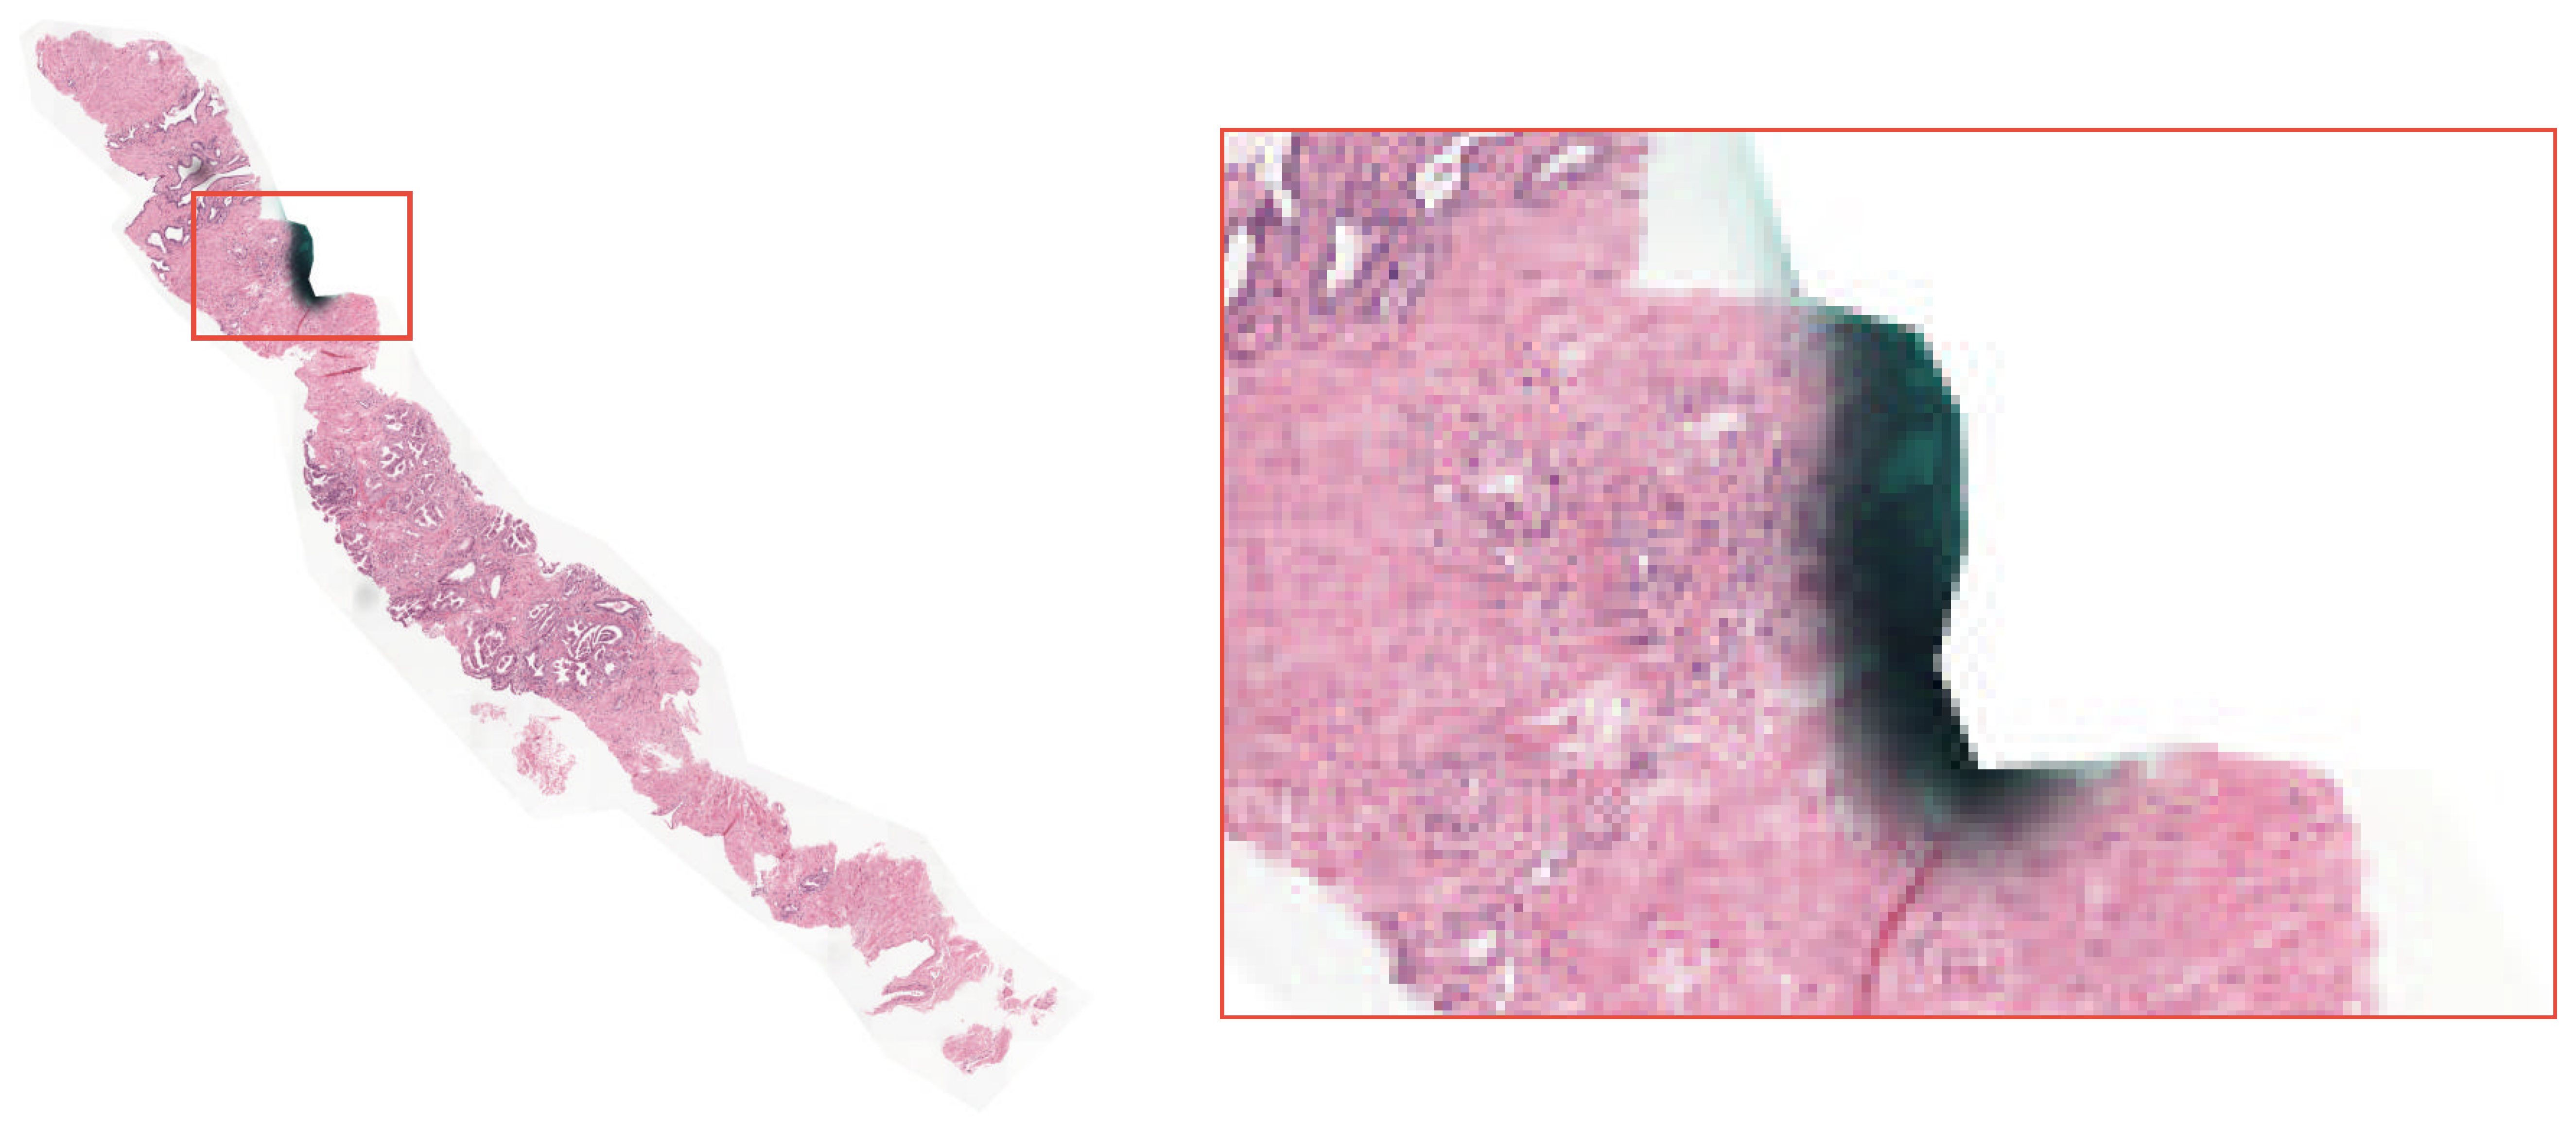
\includegraphics[width=0.8\linewidth]{images/zoom_region.png}
	\caption{Example of a visual artifact present in a WSI from the PANDA dataset.  
	On the left, the whole slide is shown with the region of interest highlighted in red.  
	On the right, a zoomed-in view of the selected region reveals a pen mark over the prostate tissue.}
	\label{fig:pen_mask}
\end{figure}

Another relevant aspect of the dataset is the uneven distribution of samples across the six grading classes (ISUP 0 to ISUP 5).  
This imbalance is evident in Table~\ref{fig:distribuicao-isup}, which presents the distribution of samples per class.  
Most examples are concentrated in the ISUP 0 and ISUP 1 classes.

\begin{figure}[htb]
	\centering
	\includegraphics[width=1\textwidth,height=0.3\textheight]{"images/distribuição ISUP"}
	\caption{Sample distribution in the PANDA dataset}
	\label{fig:distribuicao-isup}	
\end{figure}

\subsection{Preprocessing}
\label{sub:pre}

The preprocessing workflow consisted of two sequential stages: label-noise filtering and patch extraction.  
Initially, the dataset was split into training (85\%) and test (15\%), ensuring independence between model fitting and final evaluation.  
After this split, the training set contained 9,024 instances, while the test set, used for evaluating all models in this study, consisted of 1,592 instances.

\subsubsection{Entropy-Based Noise Filtering}
\label{sub:entropia}

As reported in Section~\ref{sub:data}, the PANDA dataset contains label noise due to manual annotations and inconclusive pathological reports. To mitigate its impact, a filtering strategy based on predictive uncertainty estimation was adopted.

Four low-complexity variants of the EfficientNet family (B0, B1, B2, and B3) were trained, reserving 20\% of the training set for internal validation. Each model then produced probability outputs for all training and validation samples.

Given that the network outputs independent probabilities per node via a sigmoid activation, predictive uncertainty was quantified using Shannon entropy computed directly from these outputs, without explicit class assignment \cite{ali2023entropy}. Considering $C$ as the number of output nodes and $p_c$ as the predicted probability for the $c$-th node, the mean binary entropy for a sample is defined as:

\begin{equation}
	H = \frac{1}{C} \sum_{c=1}^{C} -[p_c\log(p_c) + (1-p_c)\log(1-p_c)]
\end{equation}

Predictions with probabilities closer to 0 or 1 yield lower entropy (higher confidence), whereas values near 0.5 indicate higher uncertainty. Entropy was computed per sample for each model and then averaged across the four networks.

The top 10\% highest-entropy samples were selected as \textit{hard samples}. Their removal from the training set was evaluated under four scenarios: (i) no removal, (ii) removal of 100\%, (iii) 50\%, and (iv) 20\% of the \textit{hard samples}.
\subsubsection{Patch Extraction}
\label{sub:patches}

After defining the training samples through entropy filtering, the final preprocessing stage consisted of generating input images for the final model.  
Since the histological tissue occupies only a fraction of the WSI, as shown in Figure~\ref{fig:original-panda}, processing the full slide would require a high and unnecessary computational cost due to extensive background regions.

\begin{figure}[H]
	\centering
	
\includegraphics[width=0.8\linewidth]{images/original.png}
	\caption{Example image from the PANDA dataset showing a large tissue-free area.}
	\label{fig:original-panda}
\end{figure}

To extract informative regions from the images, a patch-based approach was adopted.  
A fixed patch size of $256 \times 256$ pixels was defined.  
To ensure standardization, white padding was applied to the WSI borders, guaranteeing exact divisibility into patches of this size.  
Then, each image was partitioned, and tissue presence was estimated by summing the RGB values of each patch; since the background tends to be white, patches with lower sums indicate higher tissue density.  
The patches were then sorted in ascending order according to this metric.  
In cases where the WSI contained insufficient tissue to reach the desired number of patches, the remaining positions were filled with white patches.

Finally, the spatial arrangement of the patches was evaluated in 5$\times$5, 6$\times$6, and 7$\times$7 configurations (Figure~\ref{fig:tiles-original}).  
The 5$\times$5 configuration omitted subtle lesion patterns, while the 7$\times$7 configuration generated high-dimensional images (1792$\times$1792) with excessive background.  
The intermediate 6$\times$6 configuration (36 patches, producing 1536$\times$1536 images) was adopted to balance preservation of tissue information, spatial coverage, and computational efficiency.

\begin{figure}[H]
	\centering
	
\includegraphics[width=0.9\textwidth]{images/tiles-original.png}	
	\caption{Illustration of patch extraction at different sizes: 5$\times$5 (left), 6$\times$6 (center), and 7$\times$7 (right).}
	\label{fig:tiles-original}
\end{figure}

\subsection{Feature Extraction and Model Training}

This section describes the strategy for training the classifiers, following the image preprocessing stage.  
Initially, the EfficientNet-B0 architecture was adopted as the base model for hyperparameter tuning due to its balance between representational capacity and computational efficiency.  
Once the optimal configuration was defined, experiments were extended to the EfficientNet-B3 and EfficientNet-B7 architectures.  
This methodological progression enabled the assessment of the impact of increased structural complexity on model performance and generalization.

During hyperparameter evaluation and baseline model construction, the BCE loss function served as the initial reference.  
Different combinations of learning rate, dropout, and proportion of unfrozen layers for \textit{fine-tuning} were investigated through a grid search using the EfficientNet-B0 architecture.  
Even after this optimization, framing the problem as conventional multiclass classification limited the model's performance.  
Considering that ISUP grades represent an ordinal progression of tumor severity, the problem was reformulated as an ordinal regression task to capture the hierarchical dependence among classes.

In this approach, ISUP grade prediction is not treated as a multiclass problem with independent categories, but rather as a sequence of cumulative binary classifications.  
For an ISUP grade $k \in \{0, \dots, 5\}$, the label is encoded as a cumulative binary vector where the first $k$ elements are set to 1 and the remaining elements to 0.  
For example, grade 3 is represented as $[1,1,1,0,0]$.  
This encoding enables the model to learn progressive thresholds associated with increasing disease severity.


To exploit this ordinal structure, a composite loss function combining two complementary terms was employed.  
The first term corresponds to Binary Cross-Entropy (BCE) applied to the cumulative thresholds.  
To address class imbalance and emphasize hard samples, this term is modulated using the focal loss mechanism.

Considering $\hat{p}_i = \sigma(z_i)$ as the predicted probability for threshold $i$, where $\sigma(\cdot)$ denotes the sigmoid function and $z_i$ represents the corresponding logit, the focal loss is defined as:

\[
\mathcal{L}_{focal} = - \frac{1}{K} \sum_{i=1}^{K}
\alpha_t (1 - p_t)^{\gamma} \log(p_t)
\]

where:

\[
p_t = \hat{p}_i y_i + (1 - \hat{p}_i)(1 - y_i)
\]

and

\[
\alpha_t = \alpha y_i + (1 - \alpha)(1 - y_i)
\]

Here, $y_i$ denotes the binary target associated with threshold $i$, $\gamma$ is the focusing parameter that reduces the contribution of easy samples, and $\alpha$ is a balancing factor between classes.

The second term introduces a penalty based on the absolute difference between the model's predicted class and the true label.  
The expected class is obtained by summing the probabilities associated with the predicted thresholds.

Formally, the estimated class is defined as:

\[
\hat{y} = \sum_{i=1}^{K} \hat{p}_i
\]

where $K$ is the number of ordinal thresholds.  
The ordinal penalty is then given by:

\[
|\hat{y} - y|
\]

where $y$ represents the ground truth class.

The final loss function is defined as:

\[
\mathcal{L} = \lambda \cdot \mathcal{L}_{focal} + \beta \cdot |\hat{y} - y|
\]

where $\lambda$ and $\beta$ control the relative contribution of the classification and ordinal penalty terms, respectively.  
This formulation preserves the ordinal structure of the problem by penalizing more severe misclassifications, while simultaneously emphasizing difficult samples through the focal mechanism.

\subsection{Performance Evaluation}

After defining the methodological pipeline, encompassing patch extraction, hyperparameter optimization, and loss function adjustment, the performance of the EfficientNet architectures (B0, B3, and B7) was evaluated on unseen data.

\subsubsection{Metrics and Statistical Analysis}

Model predictive performance was measured using Accuracy, Precision, F1-score, and Quadratic Weighted Kappa.  
Accuracy reflects the overall proportion of correct predictions \cite{baldi2000assessing}. Precision (macro-averaged) measures the proportion of correctly predicted samples among all samples predicted for each class, providing insight into the reliability of positive predictions across classes \cite{sokolova2009systematic}.  
The F1-score (macro-averaged), defined as the harmonic mean of precision and recall, balances false positives and false negatives, offering a more comprehensive evaluation in the presence of class imbalance \cite{powers2011evaluation}.

The kappa quadratic metric assesses agreement between predictions and true labels while applying penalties proportional to the magnitude of errors.  
This property makes it particularly suitable for handling the ordinal progression inherent in ISUP grading \cite{ref-cohen1968}.

To quantify uncertainty and variability in the results, a non-parametric \textit{bootstrap} method was applied \cite{efron1979bootstrap}.  
1,000 resamplings with replacement were generated from the test set predictions, preserving the original sample size.  
In each iteration, the metrics were recalculated to estimate the mean, standard deviation, and 90\% confidence interval (percentiles 5\% and 95\%).  
This strategy ensures a robust statistical assessment, independent of assumptions about the underlying data distribution.